\documentclass[mathematics,article,submit,pdftex,moreauthors]{Definitions/mdpi}
\usepackage{booktabs}
\usepackage{longtable}
\usepackage{graphicx}
\usepackage{amsmath}
\usepackage{amssymb}
\usepackage{xurl}
\setlength{\emergencystretch}{2em}
\setlength{\headheight}{25pt}
\firstpage{1}
\pubvolume{1}
\issuenum{1}
\articlenumber{0}
\pubyear{2026}
\copyrightyear{2026}
\datereceived{ }
\daterevised{ }
\dateaccepted{ }
\datepublished{ }
% Submission draft: suppress publisher-generated volume/article/DOI placeholders.
\doinum{}
\hreflink{}
\makeatletter
\renewcommand{\papercitation}{\space\@AuthorCitation\ \@TitleCitation.
Manuscript prepared for \textit{Mathematics}.}
\apptocmd{\ps@plain}{\fancyfoot[R]{}}{}{\PackageError{draftmetadata}{Could not suppress draft DOI footer}{}}
\makeatother
\Title{Functional Meaning of Kernel-Selection Weights: Normalization, Branch Interventions, and Static Simplification in 3D Segmentation}
\TitleCitation{Functional Meaning of Kernel-Selection Weights}
\Author{Jaewon Cheon $^{1,\dagger}$, Hee Kuk $^{1,\dagger}$, Zeeshan Abbas $^{2,3,4,}$* and Seung Won Lee $^{2,3,}$*}
\AuthorNames{Jaewon Cheon, Hee Kuk, Zeeshan Abbas and Seung Won Lee}
\AuthorCitation{Cheon, J.; Kuk, H.; Abbas, Z.; Lee, S.W.}
\firstnote{These authors contributed equally to this work and share first authorship.}
\address{%
$^{1}$ \quad Department of MetaBioHealth, Sungkyunkwan University, Suwon, Republic of Korea\\
$^{2}$ \quad Department of Precision Medicine, Sungkyunkwan University School of Medicine, Suwon, Republic of Korea\\
$^{3}$ \quad Department of Artificial Intelligence, Sungkyunkwan University, Suwon, Republic of Korea\\
$^{4}$ \quad Department of Biomedical Engineering, College of IT Convergence, Gachon University, Seongnam, Republic of Korea}
\corres{Correspondence: zabbas@jbnu.ac.kr (Z.A.); swleemd@g.skku.edu (S.W.L.)}
\abstract{Learned kernel-selection weights are often interpreted as indicating the importance of convolutional branches. Their functional reference, however, depends on the intervention and the operators surrounding the mixture. We analyze branch removal, renormalized removal, forced-path performance, and static simplification in a controlled three-dimensional segmentation system. A finite-epsilon identity characterizes when instance normalization attenuates removal-policy differences and when low surviving variance preserves them; a local derivative and counterexamples explain why weight magnitude alone cannot determine functional importance. Deterministic probes and direct measurements on fifteen terminal brain-tumor banks verify these operator conditions. Across five folds and three training seed groups, weight--removal associations exceed absolute weight--forced-path associations in every bank. Seed-specific pooled correlations are 0.879, 0.576, and 0.743 for removal, versus 0.094, \texorpdfstring{$-0.126$}{-0.126}, and 0.067 for forced paths. Paired removal policies differ little at the last decoder stage but by up to 0.281 region-macro Dice at the first; matched float32 sensitivity retains large differences. Separate five-fold, single-seed compact schedules reduce recorded active computation by approximately 53--58\% relative to dense multi-branch controls, without resolving a uniquely preferred schedule. These observations support an operator-aware interpretation: selection weights can describe dependence within a jointly trained mixture without identifying a sufficient path or a uniquely preferred compact architecture.}
\keyword{adaptive kernel selection; instance normalization; functional importance; computational intervention; multi-branch networks; brain tumor segmentation}
\begin{document}
\newcommand{\AnalyticResidual}{1.33e-15}
\newcommand{\ModuleResidual}{2.66e-15}
\newcommand{\ScheduleCanonicalDice}{0.902464}
\newcommand{\ScheduleAttentionDice}{0.903489}
\newcommand{\ScheduleDropDice}{0.902562}
\newcommand{\ScheduleUniformDice}{0.902626}
\newcommand{\ScheduleSKDice}{0.902913}
\newcommand{\ScheduleAttentionSavings}{55.5--58.3\%}
\newcommand{\ScheduleDropSavings}{52.9--55.7\%}


\section{Introduction}
Multi-scale convolutional systems use learned coefficients to combine
branches with different receptive fields. In Selective Kernel Networks,
channel-wise attention supports adaptive receptive fields \cite{li2019sknet}.
These explicit, inexpensive-to-record coefficients refer to named components,
making them attractive diagnostics. Interpreting them requires a specified
functional target.

Byra et al. provide a direct medical-imaging precedent: in breast-ultrasound
selective-kernel U-Net, sample-level dilated-branch attention correlated with
lesion size (Spearman coefficients around 0.7 in the early expansion-path
SK blocks) \cite{byra2020skunet}.
This association describes a learned morphological response. We ask which
functional target it reflects: removal dependence, forced-path performance,
or separately trained compact-model performance.

A large coefficient might identify a branch whose removal changes the
system, one that works well alone, or one preferable in a compact architecture.
Removal preserves the remaining fitted parameters; forced-path inference
retains one branch and the shared encoder/downstream network; compact-model
training changes the optimization problem. A \emph{static kernel schedule}
fixes one kernel per selected stage before training. Unlike fitting constant
output-mixture weights over a retained expert bank, it changes structure.
These operations require separate outcome definitions and comparisons.

Attention-interpretation studies motivate this distinction. Jain and Wallace
compare attention with functional attribution and construct alternative
distributions with similar predictions
\cite{jain2019attention}. Serrano and Smith manipulate attention in trained
predictors to relate its magnitude to prediction changes \cite{serrano2019attention}.
Wiegreffe and Pinter emphasize explanation targets and model-consistent
controls \cite{wiegreffe2019attention}. These token-attention studies motivate
precise kernel-mixture definitions without determining medical-convolutional
behavior.

The mixture is rarely the final prediction: normalization and activation
mediate downstream differences. Instance normalization centers and rescales
spatial variation independently per input and channel \cite{ulyanov2016instance},
potentially making distinct weight edits nearly equivalent. Conversely, a
small weight can multiply a large feature tensor or a strongly amplified
direction. Coefficients must therefore be examined with their operators.

We make three connected contributions: define removal dependence, forced-path
performance and independently trained kernel competence, deriving a
finite-epsilon identity and local sensitivity expression; test their operator
conditions with deterministic tensors and the unchanged selector; and verify
the analysis through terminal-checkpoint brain-tumor interventions and static
architectural simplification. The object is a kernel-selection signal within
a specified computational system.

\section{Related Work}
\subsection{Adaptive receptive fields and kernel mixtures}
CondConv and Dynamic Convolution assemble input-conditioned kernel parameters
before convolution \cite{yang2019condconv,chen2020dynamic}, unlike executing
all branches of a feature-fusion bank. CondConv uses sigmoid routing and
Dynamic Convolution simplex weights; our derivations require the stated
simplex assumptions.

Dynamic Convolution replaces trained attention aggregation with averaging,
maximum-weight selection or shuffled weights and measures classification
accuracy \cite{chen2020dynamic}. Our candidate-wise stage edits instead
measure segmentation Dice and compare removal with renormalized removal
under shared post-fusion instance normalization; compact-model training
is evaluated separately.

SK units combine branch features with channel-wise softmax weights
\cite{li2019sknet}. We implement this selection concept in a three-dimensional
U-Net \cite{ronneberger2015unet} with four branches and shared post-fusion
instance normalization. Different normalization placement, branches and task
make this a controlled characterization, not a reproduction of the original
SKNet mechanisms or performance.

Medical applications include Byra et al.'s SK-U-Net, which combines
conventional and dilated convolutions and examines attention--mass-size
associations \cite{byra2020skunet}, and ESKNet, which adds spatial and channel
recalibration, residual learning, and deep supervision for breast ultrasound
\cite{chen2024esknet}. More recently, SGDC uses an explicitly supervised
structure branch to condition spatially varying dynamic kernels and gating
\cite{shi2026sgdc}. These medical applications use different operators:
spatially varying coefficients and residual paths fall outside our simple
post-fusion per-channel equivalence. Their performance results establish
application relevance, not branch-removal evidence.

\subsection{Attention and functional attribution}
The debate on attention explanation includes correlation tests, removal
experiments, alternative weights, seed calibration, and jointly trained
adversaries \cite{jain2019attention,serrano2019attention,wiegreffe2019attention}.
These controls address different targets. We examine intervention--normalization
interactions in kernel mixtures and distinguish frozen-system dependence
from compact-model training.

Serrano and Smith zero selected token-attention weights, renormalize the
survivors, and measure output-distribution divergence and decision flips
\cite{serrano2019attention}. Our paired-policy analysis asks how subsequent
per-channel spatial normalization attenuates or preserves the difference
between removal with and without renormalization. It adds an operator
condition and trained-stage measurements to the established erasure test.

Michel et al. mask or retain single attention heads and study incremental
pruning \cite{michel2019heads}, directly preceding the removal/forced-path
distinction. We examine normalized spatial mixtures with paired removal
policies and repeated training.
Adebayo et al. use parameter and label randomization to test whether saliency
maps depend on the learned system \cite{adebayo2018sanity}, a complementary
property to removal loss or forced-path performance.

ROAR retrains image classifiers after removing ranked input pixels to reduce
confounding from the modified input distribution \cite{hooker2019roar}.
Our schedules instead change internal structure while retaining imaging
inputs. Both distinguish frozen-system edits from training a modified system.

\subsection{Normalization and representational equivalence}
Instance normalization removes instance-specific contrast in image generation
\cite{ulyanov2016instance}. From its standard definition, we derive and
verify the finite-epsilon relation governing paired branch removal and its
equivalence conditions; no new normalization operator is introduced.

Scale invariance and optimization are also linked in van Laarhoven's analysis
of weight rescaling under batch, weight, and layer normalization
\cite{vanlaarhoven2017normalization}, linking parameter scale to effective
learning rate. Here, branch removal rescales a fixed-checkpoint mixture under
per-channel spatial normalization with input-specific evaluation statistics.

Norm-based Transformer analyses already show that attention coefficients
must be considered together with transformed-vector magnitude
\cite{kobayashi2020norm}. A subsequent study incorporates residual
connections and layer normalization into the entire attention block
\cite{kobayashi2021normalization}. This established operator-aware attribution
motivates our narrower object: spatial per-channel kernel mixtures, paired
removal-policy equivalence, forced paths and separately trained static
architectures.

\section{Mathematical Formulation}
\subsection{Mixture and intervention targets}
For input $x$ at stage $s$, branch $k$ produces a tensor
$b_{s,k}(x)\in\mathbb{R}^{C_s\times V_s}$. The number of spatial positions
is $V_s$. Channel-wise weights satisfy
\begin{equation}
 a_{s,k,c}(x)\geq0,\qquad \sum_{k=1}^K a_{s,k,c}(x)=1,
 \qquad z_{s,c}(x)=\sum_k a_{s,k,c}(x)b_{s,k,c}(x).
\end{equation}
Each coefficient is constant across spatial positions within its channel.
The stage output is $u_s=\phi_s(N_s(z_s))$. Let $F$ denote the full trained
network, including all unchanged stages, and $\ell(F(x),y)$ its task loss.
Weights are generated before an edit at the chosen stage and retained for the
surviving branches. Later stages may respond to the modified representation.

For a chosen branch $k$, define the unnormalized removal mixture and the
renormalized removal mixture by
\begin{equation}\label{eq:remove}
 z_{s,c}^{-k}=\sum_{j\ne k}a_{s,j,c}b_{s,j,c},\qquad
 \widetilde z_{s,c}^{-k}=\frac{z_{s,c}^{-k}}{1-a_{s,k,c}}.
\end{equation}
The latter is defined when $a_{s,k,c}<1$. A forced-path intervention instead
uses $z_{s,c}^{[k]}=b_{s,k,c}$. For loss-based reporting, removal dependence is
\begin{equation}
 D_{s,k}(x,y)=\ell(F_{s,-k}(x),y)-\ell(F(x),y),
\end{equation}
while forced-path performance is $Q_{s,k}(x,y)=M(F_{s,[k]}(x),y)$ for a
specified higher-is-better metric $M$. Dice-based removal effects use
$M(F(x),y)-M(F_{s,-k}(x),y)$. A negative effect means that removal improved
this metric; the definition imposes no positivity assumption.

An independently trained fixed-kernel model $H_k$ has competence
$M(H_k(x),y)$. This is distinct from $Q_{s,k}$: $F_{s,[k]}$ retains a
co-adapted shared network and changes only one stage. We reserve the term
forced-path performance for the latter throughout.

\subsection{Exact relation under instance normalization}
For a vector $z\in\mathbb{R}^{V}$, let $\mu(z)$ and $v(z)$ be its spatial
mean and population variance. The non-affine normalization core is
\begin{equation}
 N_\epsilon(z)=\frac{z-\mu(z)\mathbf{1}}{\sqrt{v(z)+\epsilon}}.
\end{equation}
The following relation concerns one input and channel; its scale may differ
between channels or inputs.

\begin{Proposition}[Finite-epsilon scaling relation]\label{prop:scale}
For $\epsilon\geq0$, $t>0$, and $v(z)+\epsilon>0$,
\begin{equation}\label{eq:scale}
 N_\epsilon(tz)=r(t,v,\epsilon)N_\epsilon(z),\qquad
 r(t,v,\epsilon)=\sqrt{\frac{v+\epsilon}{v+\epsilon/t^2}}.
\end{equation}
When $\epsilon=0$ and $v>0$, the two normalized tensors are identical.
For $t\geq1$ and $v>0$,
\begin{equation}\label{eq:bound}
 0\leq r-1\leq\frac{\epsilon(1-t^{-2})}{2(v+\epsilon/t^2)}.
\end{equation}
\end{Proposition}
\begin{proof}
The mean of $tz$ is $t\mu(z)$ and its variance is $t^2v(z)$.
Substitution into $N_\epsilon$ gives Equation~\eqref{eq:scale}.
For the bound, write
$r=\sqrt{1+q}$ with
$q=\epsilon(1-t^{-2})/(v+\epsilon/t^2)\geq0$, and use
$\sqrt{1+q}-1\leq q/2$.
\end{proof}

At $v=0$ and $\epsilon>0$, $r=t$ but both normalized tensors are zero.
Thus a large scaling ratio alone does not imply a large absolute tensor
difference; the bound in Equation~\eqref{eq:bound} can also be loose at low
positive variance.

Equation~\eqref{eq:remove} supplies $t_c=(1-a_{s,k,c})^{-1}\geq1$.
Consequently, removal and renormalized removal have identical post-normalized
stage outputs in the zero-epsilon, positive-variance idealization. Applying
the same activation and downstream computation preserves this equality.
With finite epsilon, the ratio of spatial variance to epsilon determines the
remaining amplitude difference. The statement concerns the stage tensor:
a finite tensor difference does not guarantee an identical thresholded mask
or equal Dice. Downstream sensitivity and decision margins still matter.

For an affine normalization $A_\epsilon(z)=\gamma N_\epsilon(z)+\beta$,
the corresponding difference is
$\gamma(r-1)N_\epsilon(z)$; the entire affine output is not generally
multiplied by $r$. The implemented shared post-fusion normalization is
non-affine and uses input-specific statistics during evaluation.
The executable removal routine floors a positive surviving-weight denominator
at $10^{-8}$ and returns a zero mixture if no branch survives. In the floored
case, Equation~\eqref{eq:scale} uses the actual positive scale from that
routine; the unfloored expression $t=(1-a_k)^{-1}$ applies above the floor.
Spatially varying weights, normalization across multiple channels with
different $t_c$, or fixed running statistics fall outside the stated
per-channel equivalence conditions.

\subsection{Boundary under group normalization}\label{subsec:groupnorm}
Group normalization pools spatial positions and channels within each
predefined channel group \cite{wu2018groupnorm}. For one input and group $g$,
flatten its features as $z_g\in\mathbb{R}^{m_g}$ and let
$P_g=I-\mathbf{1}\mathbf{1}^{\mathsf T}/m_g$ center that group.
Renormalized removal applies a positive diagonal scale $D_g$ whose entries
repeat the channel-specific $t_c$ across spatial positions. Where the
denominator is positive, its non-affine normalized core is
\begin{equation}\label{eq:gnscale}
 \mathrm{GN}_{g,\epsilon}(D_gz_g)=
 \frac{P_gD_gz_g}{\sqrt{\|P_gD_gz_g\|^2/m_g+\epsilon}}.
\end{equation}
If every channel in the group has the same scale $t>0$, then $D_g=tI$;
substitution gives exactly Equation~\eqref{eq:scale} with the group variance
in place of the per-channel spatial variance. For unequal scales, however,
$P_gD_g\ne D_gP_g$ and the group mean is
$\mu_g(D_gz_g)=m_g^{-1}\sum_i(D_g)_{ii}(z_g)_i$.
A common factor cannot generally be extracted from the centered tensor or
its variance. This is the step at which the instance-normalization argument
ceases to apply; even at zero epsilon, the two outputs need not be proportional.
Special inputs can still yield equality.

One channel per group recovers the instance-normalization core. The
all-channel, one-group control in Figure~\ref{fig:norm}B instead combines
channels with unequal surviving-mass scales and illustrates this boundary.
The distinction is therefore the alignment of rescaling with the statistics
pool, rather than the normalization name alone. A subsequent fixed affine
transform is handled as above; the common-scale relation is a statement
about the normalized core.

\subsection{Local functional sensitivity}
Let $C=I-\mathbf{1}\mathbf{1}^{\mathsf T}/V$, $w=Cz$, and
$q=\sqrt{\|w\|^2/V+\epsilon}$. On the domain $q>0$, differentiation yields
\begin{equation}\label{eq:derivative}
 DN_\epsilon(z)[h]=\frac{Ch}{q}
 -\frac{w\langle w,Ch\rangle}{Vq^3}.
\end{equation}
In particular,
\begin{equation}
 DN_\epsilon(z)[z]=\frac{\epsilon Cz}{(v+\epsilon)^{3/2}}.
\end{equation}
For a group-normalized core, Equation~\eqref{eq:derivative} has the same
form after replacing $C,V$ by $P_g,m_g$. A relative channel rescaling gives
$h=Az_g$, with diagonal $A$; this direction need not lie in that derivative's
null space even at zero epsilon. For instance normalization,
at zero epsilon and positive variance, infinitesimal common scaling lies in
the normalization derivative's null direction. The equation describes the
geometry of the operator; it does not imply that removing a branch is merely
common scaling, since removal also changes the mixture's direction.

For a weight transfer from branch $j$ to branch $k$, hold the selected-stage
branch tensors fixed and choose $\delta a$ so that the coefficients remain
in the simplex; at its boundary only admissible directions are considered.
Then $\delta z=\delta a(b_k-b_j)$. Assume $q>0$ and that both $\phi$ and the
downstream loss are differentiable at the evaluated representation, excluding
activation kinks. The first-order change is
\begin{equation}\label{eq:local}
 \delta\ell=\delta a\left\langle\nabla_u\ell,
 D\phi(N_\epsilon(z))DN_\epsilon(z)[b_k-b_j]\right\rangle
 +o(|\delta a|).
\end{equation}
The downstream gradient includes the response of subsequent stages; their
selectors are not frozen by the selected-stage edit.
Weight magnitude does not specify the branch difference, normalization
Jacobian, or downstream loss gradient. A full removal or forced-path edit is
a finite intervention and need not be approximated well by this derivative.
For thresholded Dice, which is not differentiable in the required sense,
Equation~\eqref{eq:local} motivates the distinction but is not used to
calculate the reported effects.

\subsection{Coefficient magnitude does not order forced-path performance}
\begin{Example}[Cancellation with positive simplex weights]\label{ex:counter}
Consider an identity readout, squared loss, target $y=0$, coefficients
$(0.6,0.3,0.1)$, and scalar branch values $(5,0,-30)$. The mixture equals zero
and has zero loss. Forced-path losses are $(25,0,900)$, so the largest-weight
branch is not the best forced path. Unnormalized removal losses are $(9,0,9)$,
so the smallest-weight branch has the same removal effect as the
largest-weight branch.
\end{Example}
This construction excludes a universal coefficient ordering of either target,
without estimating cancellation prevalence in medical networks. Interpretation
requires branch features and a downstream target. Segmentation branches are
spatial features, not calibrated tumor probabilities: their mixture passes
through normalization, activation and a shared decoder. The scalar identity
readout isolates cancellation without spatial normalization or anatomical
kernel assignments. We therefore assess removal and forced-path Dice within
the actual normalized network, and independently train fixed schedules to
assess compact-model performance. Shared branch names do not equate these
three operations.

\begin{Example}[Cancellation in normalized spatial features]\label{ex:featuremaps}
Consider two intermediate feature maps,
\[
 u=\begin{pmatrix}1&-1\\0&0\end{pmatrix},\qquad
 v=\begin{pmatrix}0&0\\1&-1\end{pmatrix}.
\]
Each has zero mean and variance $1/2$, and their inner product is zero.
Use branch maps $(5u,v,-30u)$ and weights $(0.6,0.3,0.1)$. Their mixture
is $0.3v$. Apply the non-affine instance-normalization core with zero
epsilon, followed by an identity readout, and set the feature target to
$y=N_0(v)$. With loss $\ell(z)=\|N_0(z)-y\|^2/4$, the mixture loss is
zero and forced-path losses are $(2,0,2)$. All normalized maps in this
comparison have positive variance. The largest-weight branch is therefore
not the best forced path even after spatial normalization.
\end{Example}
Example~\ref{ex:featuremaps} extends the scalar construction to spatial
normalization. Its normalized-feature target and squared-error loss are
neither MRI observations nor Dice, and assign no anatomical kernel role.

\section{Materials and Methods}
\subsection{Numerical verification}
We implemented Equation~\eqref{eq:scale} with float64 tensors and a fixed
random seed of 20261001. The variance-to-epsilon ratio spans $10^{-6}$ to
$10^8$ at 71 logarithmically spaced points; scales are 1.1, 2, and 8, with
$\epsilon=10^{-5}$. Centered tensors are rescaled to the specified population
variance before each comparison. The residual is the maximum absolute
difference between direct normalization and the analytic prediction.

A second experiment fixes branch tensors and weight edits while changing
only the surrounding operator: post-fusion instance normalization with
epsilon zero or $10^{-5}$, no post-fusion normalization, branch-local
normalization only, group normalization across all channels, and spatially
varying coefficients followed by instance normalization. Twelve seeded
tensor trials use two instances, four branches, four channels, and a
$5\times6\times7$ spatial grid. We report the relative tensor norm change
between removal and renormalized removal.

We also evaluate the unchanged SK selector on twelve small CPU inputs,
using deterministic random head weights rather than uniform initialization.
Replacing activation by identity only in this probe verifies the
pre-activation finite-epsilon relation. These numerical controls leave trained
models and checkpoints unchanged.

\subsection{Brain-tumor cohort and common training}
Medical-imaging experiments use the BraTS 2023 adult glioma training cohort
\cite{bakas2023cluster,menze2015brats}. Our data manifest contains 1,251 studies
from 1,133 patients, including 118 patients with two studies. A fixed five-fold partition groups
studies by patient. The primary stage study evaluates all five folds for
three base seeds (S1: 2026; S2: 20261001; S3: 20261011), using base seed plus
fold index: fifteen terminal banks on the same 1,251 studies, not independent
cohorts. The historical schedule study used folds 0--2 (751 studies,
679 patients); a retrospective missing-fold extension completes five-fold
schedule and final-block pooling comparisons, each still single-base-seed.
The separate single-configuration architecture matrix also covers five folds.

S1 and schedule-study SK share base seed 2026 and recorded scientific settings,
but use separately trained checkpoints: new folds 0--4 versus historical
folds 0--2 plus the later extension. Appendix~\ref{app:reporting} compares
their scores and provenance; nominal seed/recipe agreement does not establish
bitwise training equivalence.

A separate routing manuscript in preparation shares this cohort,
preprocessing, patient folds and historical fixed-kernel infrastructure.
It addresses complete-expert competence, case-level role reproducibility and
adaptive/static output policies; this paper addresses kernel interventions,
normalization and static schedules. The fifteen new banks are not routing-paper
replicas, nor are shared patients/models independent cross-paper validation.
Each paper establishes its primary findings independently.

Four MRI modalities are cropped using the union of their nonzero anatomy
plus a four-voxel margin and padded to $192\times224\times192$ without
truncating the anatomical crop. Labels do not set crop bounds. Each modality
is standardized within its nonzero support and clipped to $[-5,5]$.
Atomic labels are converted to whole tumor (WT), tumor core (TC), and
enhancing tumor (ET). The common recipe uses full volumes, batch size four,
the GPU augmentation specified in Appendix~\ref{app:augment}, binary
cross-entropy plus batch Dice, AdamW with
learning rate $2\times10^{-4}$ and weight decay $10^{-5}$, cosine decay,
100 epochs, and bfloat16 training. Terminal checkpoints provide the primary
evaluation. The evidence manifest compares versioned and actual configurations;
all twenty-five schedule model--fold records agree on non-path fields.
Appendix~\ref{app:reporting} links recipes, terminal evaluations and FLOPs.

Table~\ref{tab:architecture} specifies the common backbone and selector
locations. All backbone and post-fusion InstanceNorm3d layers use
$\epsilon=10^{-5}$, \texttt{affine=False}, and
\texttt{track\_running\_stats=False}: evaluation uses the current input's
spatial statistics, not accumulated training statistics. LeakyReLU has
negative slope 0.01. The selector replaces the second convolution,
normalization, and activation of an indicated decoder block, leaving its
first convolution and skip connection unchanged.
\begin{table}[H]
\caption{Common U-Net architecture and full-volume selector resolutions.
Spatial dimensions refer to the preprocessed input, not random patches.}
\label{tab:architecture}
\centering\small
\begin{tabular}{p{0.24\linewidth}p{0.68\linewidth}}
\toprule Component & Implementation \\
\midrule
Input and output & Four MRI channels; three output logits (WT/TC/ET). \\
Encoder & Five levels with channels 32, 64, 128, 256, 512; two bias-free
$3^3$ convolutions per level, each followed by InstanceNorm and LeakyReLU. \\
Down/up sampling & Four stride-two max pools; four $2^3$, stride-two
transposed convolutions and concatenated encoder skips. \\
Decoder and head & Channels 256, 128, 64, 32; two convolution--norm--activation
blocks before replacement; final $1^3$ convolution. \\
Selector positions & Decoder 1: $128\times48\times56\times48$;
decoder 2: $64\times96\times112\times96$;
decoder 3: $32\times192\times224\times192$ (channels $\times$ spatial shape). \\
SK selector & Sum branch features, global average pooling, hidden width
$\max(8,C/4)$, ReLU, four channel-wise heads and branch softmax.
Avg+max concatenates average and maximum pooled features. \\
\bottomrule
\end{tabular}
\end{table}

\subsection{Branches, stages, and functional measurements}
The branch bank contains dense $3^3$, $5^3$, dilation-two $3^3$, and
$1\times3\times3$ anisotropic convolutions. Branches have no local
normalization; shared instance normalization and a leaky rectifier follow
fusion. Multi-stage SK inserts selectors at decoder indices 1, 2, and 3.
SK produces channel-wise weights from pooled fused branch features; the
separately reported final-block dense-soft variant produces scalar weights
from pooled shared input.

At each selected stage, every branch is removed, removed with renormalization,
or forced alone on the same terminal checkpoint and validation studies;
other stages compute normally. Weights are averaged over channels, then
studies. The positive-reference region-macro endpoint averages study Dice
over present references within each region, then equally over three regions.
Spearman correlations use twelve stage--branch cells per fold;
Appendix~\ref{app:stage} disaggregates four-branch within-stage correlations
and functional/weight ranges using the same cells and endpoint.
Retrospective stage sensitivities residualize within-bank ranks on stage
indicators, rank branches independently within each stage, and omit each
stage in turn. We compare signed weight--removal association with absolute
weight--forced-path association (definitions/exceptions in
Appendix~\ref{app:stage}). Taking the latter's absolute value counts a negative
association as a competing signal of equal magnitude, although it opposes
the interpretation that larger weights identify better forced paths. This
sets a hurdle at least as high as a signed-to-signed comparison for the
positive removal association. These and the 60-cell seed-specific pooled
correlations are descriptive: folds share training data and stages a fitted
network, precluding independent-replica or patient-selection interpretations.
Cross-seed winner agreement compares maximum mean weight, removal effect or
forced-path Dice in 15 matched fold--stage pairs, resolving ties by fixed
branch order. This measures bank-level, not patient-level, ranking stability.

\subsection{Direct checkpoint-normalization measurements}\label{subsec:checkpointnorm}
Observation-only hooks capture selected-stage pre-normalization mixtures and
post-normalization/pre-activation outputs for paired removals on all fifteen
banks. Full-cohort evaluation preserves BF16 autocast, batch size four and
batch membership. Fidelity checks show identical observed/unobserved repeats
and historical Dice; paired stage inputs, branch tensors and pre-edit weights
must match. Measurements comprise surviving mass, denominator-floor events,
variance/epsilon and residuals of $\widetilde z=tz$ and
Equation~\eqref{eq:scale}. Fixed captured features are replayed in float64
at epsilon zero, $10^{-8}$, $10^{-5}$ and $10^{-3}$, without checkpoint edits.

A matched sensitivity selects, before inference, the first two patients per
fold ordered by SHA-256 of a protocol-specific prefix and patient ID. All
their studies give ten patients/eleven studies, reused across three seeds.
Fresh BF16 and full FP32 runs use batch size one with TF32 disabled.
They change upstream representations as well as normalization arithmetic;
only fixed-feature local replay isolates epsilon. This post-result audit
does not enlarge the patient sample through channels or repeated seeds.

\subsection{Static kernel schedules and uncertainty}
Two compact architectures were derived during the earlier 30-epoch
investigation: an attention-derived anisotropic/anisotropic/$3^3$ schedule
and a drop-derived dilated-$3^3$/$3^3$/$3^3$ schedule at decoder indices
1/2/3. Each was subsequently trained for 100 epochs on folds 0--2 and
compared with multi-stage SK, multi-stage uniform fusion, and canonical
U-Net under the same nominal recipe. The later thirteen-fit extension adds
folds 3--4 to both schedules, multi-stage SK, multi-stage uniform and GAP
dense-soft, and folds 2--4 to average-plus-maximum dense-soft. The completed
schedule comparison uses five models on five folds, base seed 2026 and
effective seed $2026+f$. This completes fold coverage, not three-seed
replication. Schedule construction used the original folds and extension
followed result inspection, making it a discovery/internal-repetition study.

We recalculate paired intervals from terminal study-level outputs using
4,000 patient-cluster bootstrap draws within each fold, with seed 20261001.
Both studies from a sampled repeated-study patient receive the same
multiplicity. Each draw recomputes positive-reference region means and then
the equal-fold mean. Explicitly, let $I_{fir}$ indicate a positive reference
for study $i$, region $r$, and fold $f$, and let $d_{mfir}$ be its Dice for
model $m$. If $w_{fi}^{(b)}$ is the bootstrap multiplicity of study $i$'s
patient, the draw-level score and paired contrast are
\begin{equation}\label{eq:bootstrap}
 S_m^{(b)}=\frac{1}{3F}\sum_{f=1}^{F}\sum_{r\in\{\mathrm{WT,TC,ET}\}}
 \frac{\sum_i w_{fi}^{(b)} I_{fir}d_{mfir}}
      {\sum_i w_{fi}^{(b)} I_{fir}},\qquad
 \Delta_{mn}^{(b)}=S_m^{(b)}-S_n^{(b)},\quad F=5.
\end{equation}
Models share sampled patients and multiplicities; paired-contrast percentiles
2.5 and 97.5 define the 95\% interval. Study IDs/reference-presence flags
match across all five models, with no missing predictions; zero eligible
denominators raise an error. Unit multiplicities give the point estimate.
Equal fold and WT/TC/ET weighting yield eligible-region study means, not a
pooled patient-weighted score; Appendix~\ref{app:reporting} lists study/patient
denominators. Intervals condition on fitted models, neither quantifying
retraining variability nor proving equivalence. Active FLOPs describe the
full-volume profile, not latency.
The repository profiler uses THOP 0.1.1 (environment lock build
\texttt{0.1.1.post2209072238}), in evaluation mode on one float32 input of
shape $1\times4\times192\times224\times192$, with
$\mathrm{FLOPs}=2\times\mathrm{MACs}$. Dense SK and uniform fusion execute
every branch, so their active and total counts coincide; a compact fixed
schedule constructs and executes only its chosen branch at each selector.
Counts follow THOP's operator-accounting convention, not measured hardware
instructions or training cost.
Recorded counts differ between the historical and later profiling regimes
by a common 0.443925 TFLOPs across these five families despite the same
reported shape and counting rule. We retain the observed ranges and compute
reductions against the same-fold dense comparator, rather than presenting
these records as harmonized re-profiling. The offset exactly matches
output-grid versus input-grid operation counting for the four stride-two
transposed convolutions; this arithmetic match does not establish which
profiler version was imported in each historical run.

During the preparation of this work, the authors used OpenAI Codex and ChatGPT
for software development, analysis support, and manuscript preparation.
The authors reviewed and edited the outputs and take full responsibility
for the content of this publication.

\section{Results}
\subsection{Numerical identity and architectural boundaries}
Maximum absolute finite-epsilon residuals are \texttt{\AnalyticResidual}
on the float64 variance/scale grid and \texttt{\ModuleResidual} in the
executable selector. Figure~\ref{fig:norm} shows accurate approximate
equivalence at ordinary variance and failure near epsilon. Zero-epsilon
per-channel post-fusion normalization cancels common positive rescaling;
removing it, moving it to branches, pooling differently scaled channels or
using spatial weights generally does not.

\begin{figure}[H]
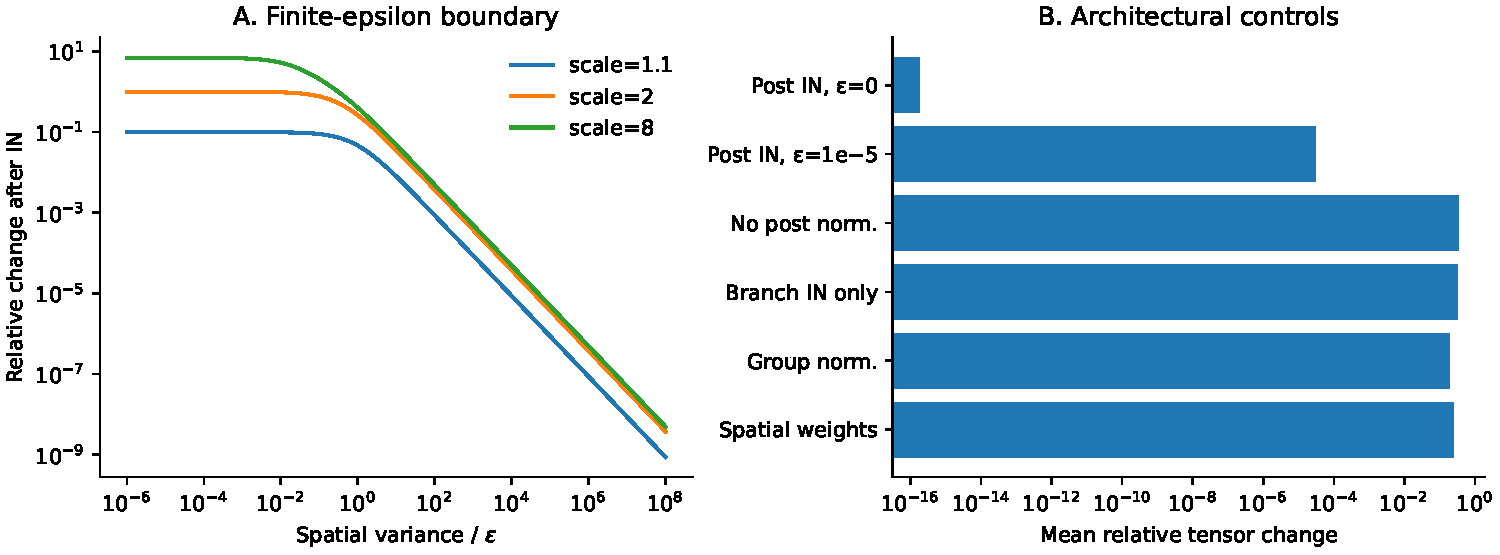
\includegraphics[width=\linewidth]{generated/normalization.pdf}
\caption{Numerical verification of removal-policy equivalence.
\textbf{A}: Relative change after instance normalization versus spatial
variance divided by epsilon, for three positive scales.
\textbf{B}: Mean relative tensor change across twelve trials under controlled
operator changes. The group-normalization control pools all four channels
in one group; Section~\ref{subsec:groupnorm} explains why unequal channel
scales prevent the per-channel argument from applying.
Zero-epsilon post-fusion instance normalization approaches
floating-point precision; the other conditions identify boundaries of the
per-channel constant-scale argument.}
\label{fig:norm}
\end{figure}

\subsection{Trained checkpoints expose the finite-epsilon boundary}\label{subsec:normresults}
The full-cohort audit reconstructs all 180 stage--branch endpoints and their
paired channel measurements without changing the original predictions.
Table~\ref{tab:checkpointnorm} shows strong stage dependence. Across sixty
cells per stage, median absolute removal-policy differences are
$1.58\times10^{-4}$, $1.14\times10^{-6}$ and $4.40\times10^{-7}$ Dice
at decoder stages 1, 2 and 3, respectively. The corresponding maxima are
0.280635, 0.000376 and 0.000019. Thus, small typical differences do not
justify treating the two policies as equivalent throughout the network.
At stage 1, absolute differences exceed 0.001, 0.01 and 0.05 in
17/60 (28.3\%), 6/60 (10.0\%) and 3/60 (5.0\%) cells, respectively;
no stage-2 or stage-3 cell exceeds 0.001. The three differences above 0.05
occur in separate seeds and folds, all for the dilated branch
(Appendix~\ref{app:normdiagnostics}). These are descriptive experiment-cell
frequencies, not patient-level event rates.
The largest full-cohort difference occurs for removal of the dilated branch
at stage 1 in S1/fold 0: unnormalized removal gives 0.816314 Dice and
renormalized removal 0.535680. The matched batch-one precision subset
retains a stage-1 maximum difference of approximately 0.40 under both
BF16 and FP32, contradicting a solely BF16 explanation.

\begin{table}[H]
\caption{Direct checkpoint comparison of removal policies on fifteen banks.
$\Delta$ is renormalized-removal minus unnormalized-removal
positive-reference region-macro Dice; each entry summarizes sixty
seed--fold--branch cells at one stage. Primary results use the full cohort
and original batch-four BF16 runtime. Subset columns use the same ten
patients/eleven studies in batch-one BF16 and FP32, not a full-cohort FP32 test.
The lower panel reports full-cohort strict exceedances, $n/60$ (percentage),
at three retrospectively chosen descriptive thresholds.}
\label{tab:checkpointnorm}
\centering\small\setlength{\tabcolsep}{3pt}
\begin{tabular}{lrrrr}
\toprule
Decoder & Primary median $|\Delta|$ & Primary max $|\Delta|$ & Subset BF16 max & Subset FP32 max \\
\midrule
1 & 1.58e-04 & 0.280635 & 0.400841 & 0.402439 \\
2 & 1.14e-06 & 0.000376 & 0.000301 & 0.000364 \\
3 & 4.40e-07 & 0.000019 & 0.000103 & 0.000082 \\
\bottomrule
\end{tabular}

\par\medskip
\begin{tabular}{lrrr}
\toprule
Decoder & $|\Delta|>0.001$ & $|\Delta|>0.01$ & $|\Delta|>0.05$ \\
\midrule
1 & 17/60 (28.3\%) & 6/60 (10.0\%) & 3/60 (5.0\%) \\
2 & 0/60 (0.0\%) & 0/60 (0.0\%) & 0/60 (0.0\%) \\
3 & 0/60 (0.0\%) & 0/60 (0.0\%) & 0/60 (0.0\%) \\
\bottomrule
\end{tabular}

\end{table}

At stage 1, low surviving variance/epsilon permits near-unit post-normalization
RMS differences despite nearly proportional input mixtures. Finite-epsilon
predictions closely match the outputs, and fixed-feature zero-epsilon replay
largely removes the difference. Appendix~\ref{app:normdiagnostics} reports
channel counts, variance ranges, floor events and residuals. This verifies
the captured-stage mechanism, not individual-channel attribution of final
Dice or every downstream amplification mechanism.

\subsection{Weights track removal dependence more than forced paths}
Table~\ref{tab:stage} reconstructs all fifteen banks' terminal correlations. Weight--removal
correlations are positive in every bank ($\rho=0.252$--$0.951$) and exceed
the absolute weight--forced-path correlation in every bank
($|\rho|\leq0.273$). The descriptive pooled removal associations are
0.879, 0.576, and 0.743 for S1, S2, and S3, respectively; forced-path associations are
0.094, $-0.126$, and 0.067: the distinction repeats with seed-dependent
strength. Figure~\ref{fig:intervention} displays the cells; global correlations
do not imply exact study-specific rankings. Similar paired removal correlations
also do not imply tensor/mask equivalence, given the stage-1 exceptions in
Section~\ref{subsec:normresults}. Forced paths change mixture content and
test a different target.

Within-stage removal association is positive in 41 of 45 fold--stage cells
(range $-0.6$ to 1.0), while forced-path associations have both signs
(Appendix~\ref{app:stage}). These descriptive four-branch correlations show
heterogeneous stage-specific ranking strengths. Removal-effect ranges also
differ: similar correlations do not imply equal effects.

After residualizing ranks on stage indicators, removal associations remain
positive and exceed absolute forced-path associations in all fifteen banks
($\rho_{\mathrm{removal}}=0.230$--$0.966$). Independently ranking the four
branches within each stage retains the contrast in 14/15 banks. Omitting
stages 1, 2, or 3 retains it in 13/15, 15/15, and 14/15 banks, respectively;
removal association stays positive throughout (Table~\ref{tab:stagesensitivity}).
The overall distinction thus persists without uniform within-stage rankings.

Equal-fold mean Dice is 0.904036, 0.902962, and 0.902774 for S1--S3.
Across the 15 matched fold--stage groups, all three seeds identify the same
highest-weight branch in 9/15 groups, the same largest-removal-effect branch
in 11/15, and the same best forced path in 6/15. Pairwise agreement counts
for S1/S2, S1/S3, and S2/S3 are respectively 9/15, 13/15, and 11/15 for
weight; 12/15, 13/15, and 11/15 for removal; and 12/15, 7/15, and 7/15 for
forced paths. These counts show partial, target-dependent ranking
reproducibility, not a universally stable or unstable named-kernel preference.

\begin{table}[H]
\caption{Spearman association between stage--branch mean weights and
functional measurements on terminal multi-stage SK checkpoints. There are
twelve cells per bank and 60 cells in each seed-specific pooled row.
Rows S1/0--4, S2/0--4, and S3/0--4 identify base seeds 2026, 20261001, and 20261011 and folds
0--4. Pooled rows are descriptive summaries, not independent replicates.}
\label{tab:stage}
\centering\begin{tabular}{lrrr}
\toprule
Fold & Drop & Renormalized drop & Keep-one \\
\midrule
S1/0 & 0.951 & 0.937 & 0.021 \\
S1/1 & 0.783 & 0.594 & 0.105 \\
S1/2 & 0.944 & 0.902 & -0.028 \\
S1/3 & 0.909 & 0.909 & 0.021 \\
S1/4 & 0.734 & 0.706 & 0.042 \\
S2/0 & 0.252 & 0.252 & -0.203 \\
S2/1 & 0.552 & 0.573 & -0.238 \\
S2/2 & 0.790 & 0.762 & -0.147 \\
S2/3 & 0.587 & 0.559 & -0.224 \\
S2/4 & 0.804 & 0.797 & -0.007 \\
S3/0 & 0.503 & 0.503 & -0.021 \\
S3/1 & 0.664 & 0.664 & 0.007 \\
S3/2 & 0.804 & 0.741 & 0.273 \\
S3/3 & 0.944 & 0.944 & -0.119 \\
S3/4 & 0.734 & 0.734 & -0.077 \\
\midrule
S1 pooled & 0.879 & 0.842 & 0.094 \\
S2 pooled & 0.576 & 0.562 & -0.126 \\
S3 pooled & 0.743 & 0.755 & 0.067 \\
\bottomrule
\end{tabular}

\end{table}

\begin{figure}[H]
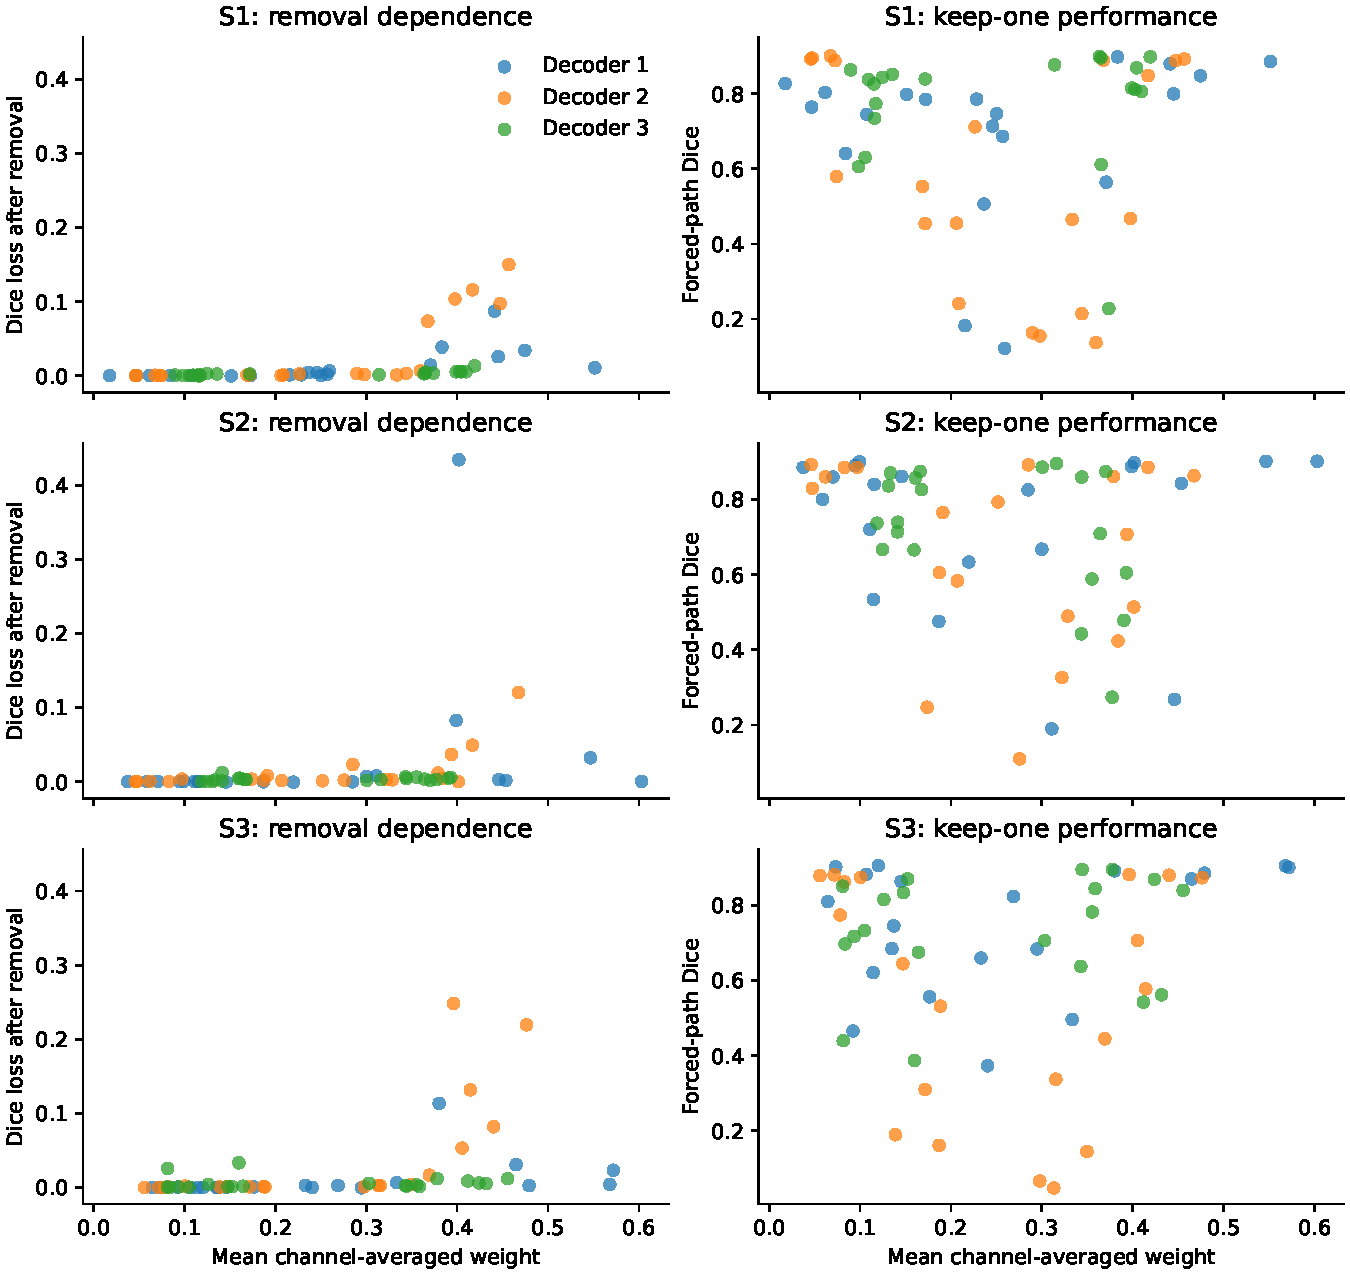
\includegraphics[width=\linewidth]{generated/interventions.pdf}
\caption{Mean weight and two functional references on the same SK banks.
Rows separate the three base-seed groups. Each point is one
fold--stage--branch cell; colors distinguish decoder
stages. Removal dependence and forced-path Dice exhibit different relations
with the recorded coefficients. The points are grouped measurements,
not independent patients or retraining replicas.}
\label{fig:intervention}
\end{figure}

In the historical three-fold study, the earlier and terminal training horizons also favor different named
stage schedules. The 30-epoch attention-derived schedule is
anisotropic/anisotropic/$3^3$, whereas terminal mean attention favors
dilated-$3^3$/dilated-$3^3$/anisotropic. Terminal mean forced-path Dice
favors dilated-$3^3$/$5^3$/$5^3$. These are distinct summaries of a
changing trained system rather than a single identified kernel assignment.

\subsection{Static simplification and its comparator}
The completed five-fold schedule comparison is reported in
Table~\ref{tab:schedules}. Equal-fold Dice is \ScheduleAttentionDice{} for
the attention-derived schedule, \ScheduleDropDice{} for the drop-derived
schedule, \ScheduleSKDice{} for multi-stage SK, \ScheduleUniformDice{} for
uniform fusion and \ScheduleCanonicalDice{} for canonical U-Net.
The SK value here belongs to the separate schedule-study bank, not the
S1 replication bank (0.904036); Appendix~\ref{app:reporting} gives the
run-level correspondence.
Relative to the dense multi-branch profiles of 8.56--9.00 TFLOPs per volume,
attention-derived and drop-derived schedules record 3.57--4.01 and
3.79--4.24 TFLOPs, respectively. Same-fold recorded reductions are
\ScheduleAttentionSavings{} and \ScheduleDropSavings{}.
Canonical U-Net records 3.79--4.24 TFLOPs, so the savings are chiefly relative to retaining multiple dense
branches at each selected stage. The result does not establish that the
diagnostic derivation found a uniquely superior compact model.

\begin{table}[H]
\caption{Completed five-fold, 100-epoch, single-base-seed static schedule study. Dice is the equal-fold
mean of study-wise positive-reference region-macro Dice. Parameters and
active FLOPs are read from the associated run artifacts. FLOP ranges retain
the historical/later profile discrepancy described in Materials and Methods.}
\label{tab:schedules}
\centering\begin{tabular}{lrrr}
\toprule
Family & Dice & Parameters (M) & Active TFLOPs \\
\midrule
Canonical U-Net & 0.902464 & 22.58 & 3.79--4.24 \\
Attention-derived fixed & 0.903489 & 22.21 & 3.57--4.01 \\
Drop-derived fixed & 0.902562 & 22.58 & 3.79--4.24 \\
Multi-stage uniform & 0.902626 & 26.04 & 8.56--9.00 \\
Multi-stage SK & 0.902913 & 26.07 & 8.56--9.00 \\
\bottomrule
\end{tabular}

\end{table}

\begin{table}[H]
\caption{Recomputed paired patient-cluster sensitivity for static
simplification. Intervals condition on stored models and preserve the
original region-macro endpoint. No non-inferiority margin was specified.}
\label{tab:contrasts}
\centering\small\begin{tabular}{lrr}
\toprule
Comparison & Difference & Conditional 95\% interval \\
\midrule
Attention-derived fixed $-$ Multi-stage SK & +0.000576 & [-0.000842, +0.002145] \\
Drop-derived fixed $-$ Multi-stage SK & -0.000351 & [-0.002279, +0.001669] \\
Attention-derived fixed $-$ Canonical U-Net & +0.001025 & [-0.000387, +0.002564] \\
Drop-derived fixed $-$ Canonical U-Net & +0.000098 & [-0.001515, +0.001822] \\
Multi-stage SK $-$ Multi-stage uniform & +0.000287 & [-0.001324, +0.001854] \\
\bottomrule
\end{tabular}

\end{table}

Table~\ref{tab:contrasts} adds patient clustering to the original study-row
bootstrap. Small differences and their intervals leave the preferred compact
schedule unresolved. The separate five-fold single-configuration matrix also
contains closely performing fixed/adaptive models; its terminal metrics
provide architectural context in the manifest, not additional three-seed
intervention replicas.

\subsection{Selector information and functional reference}
The supporting five-fold, 100-epoch, single-base-seed final-block dense-soft
comparison is rebuilt in Table~\ref{tab:pooling}. Average-plus-maximum pooling
increases study-level weight variation in all five folds. Equal-fold mean
weight SD increases from 0.00159 to 0.04807, and the mean branchwise
weight--removal correlation from 0.004 to 0.224; the correlation increases
in four of five folds, not uniformly. Mean top-weight/forced-path winner
agreement rises from 0.64\% to 9.02\%, but the average-plus-maximum values
range from 0 to 23.5\%: increased selector variation/alignment does not ensure
correct forced-path ordering. Functional correlations and winner agreement
use study-wise available-region Dice; model scores use region-macro Dice,
with both reductions retained separately. Ties use the first maximum in fixed
branch order. Historical GAP intervention baselines differ from terminal
validation by at most $1.43\times10^{-5}$; both are retained, but effects
use their own paired intervention baseline.

\begin{table}[H]
\caption{Rebuilt supporting pooling comparison. Weight SD is the mean
over branches of the across-study population standard deviation. The
weight--drop column averages four branchwise Spearman correlations.
Winner agreement compares largest weight and highest forced-path
available-region Dice on each study.}
\label{tab:pooling}
\centering\small\begin{tabular}{lrrrrr}
\toprule
Pooling & Fold & Dice & Weight SD & Weight--drop $\rho$ & Winner agreement \\
\midrule
GAP & 0 & 0.900315 & 0.00188 & -0.043 & 0.4\% \\
GAP & 1 & 0.907862 & 0.00155 & 0.101 & 0.4\% \\
GAP & 2 & 0.903934 & 0.00186 & -0.067 & 0.8\% \\
GAP & 3 & 0.902920 & 0.00089 & 0.087 & 0.4\% \\
GAP & 4 & 0.898734 & 0.00178 & -0.059 & 1.2\% \\
Average + maximum & 0 & 0.903226 & 0.05531 & 0.344 & 23.5\% \\
Average + maximum & 1 & 0.905870 & 0.05566 & 0.391 & 7.2\% \\
Average + maximum & 2 & 0.907032 & 0.03476 & 0.120 & 1.2\% \\
Average + maximum & 3 & 0.904282 & 0.04004 & 0.014 & 0.0\% \\
Average + maximum & 4 & 0.899314 & 0.05458 & 0.253 & 13.2\% \\
\bottomrule
\end{tabular}

\end{table}

\subsection{Sensitivity to absent-region false positives}
An all-case sensitivity scores every region of every study, assigning one
to empty-reference/empty-prediction pairs and zero to empty-reference/nonempty
pairs. Present-region Dice is unchanged. This makes absent-region false
positives visible, while introducing a convention for correct empty
predictions. Table~\ref{tab:fpstage} shows that weight--removal associations
remain positive, while forced-path associations remain substantially weaker.
The static-schedule contrasts in Appendix~\ref{app:fp} likewise retain
intervals spanning zero. These checks support the distinction between the
functional targets under both scored endpoints; they do not equate Dice
with clinical utility or quantify the volume of absent-region false positives.

\begin{table}[H]
\caption{Stage-level endpoint sensitivity. Spearman correlations use the
same twelve cells per fold as Table~\ref{tab:stage}.}
\label{tab:fpstage}
\centering\small\begin{tabular}{lrrr}
\toprule
Fold & Positive-ref. drop & All-case drop & All-case keep \\
\midrule
S1/0 & 0.951 & 0.944 & 0.021 \\
S1/1 & 0.783 & 0.888 & 0.105 \\
S1/2 & 0.944 & 0.944 & -0.014 \\
S1/3 & 0.909 & 0.797 & 0.021 \\
S1/4 & 0.734 & 0.629 & 0.042 \\
S2/0 & 0.252 & 0.385 & -0.203 \\
S2/1 & 0.552 & 0.566 & -0.238 \\
S2/2 & 0.790 & 0.741 & -0.147 \\
S2/3 & 0.587 & 0.643 & -0.224 \\
S2/4 & 0.804 & 0.538 & 0.014 \\
S3/0 & 0.503 & 0.545 & -0.021 \\
S3/1 & 0.664 & 0.448 & 0.070 \\
S3/2 & 0.804 & 0.853 & 0.273 \\
S3/3 & 0.944 & 0.867 & -0.189 \\
S3/4 & 0.734 & 0.573 & -0.154 \\
\bottomrule
\end{tabular}

\end{table}

\section{Discussion}
\subsection{Interpreting a weight requires an operator and a target}
Equation~\eqref{eq:local} separates the coefficient, branch-feature direction
and amplitude, and downstream sensitivity. Normalization removes one class
of variation while preserving centered-direction changes, allowing useful
weight--removal association to coexist with poor weight--forced-path association.

A branch may be necessary in a co-adapted mixture yet weak alone, or strong
alone yet redundant in the mixture. The counterexamples exclude universal
coefficient ordering of either target. Brain-tumor results demonstrate these
distinctions under the implemented normalization/readout; rank adjustments
and most stage exclusions retain the contrast while exposing local exceptions.

\subsection{Finite epsilon makes removal-policy redundancy stage-dependent}
Post-fusion instance normalization attenuates positive per-channel rescaling
when surviving variance is large relative to epsilon and the edits preserve
proportionality. Paired removals then provide nearly redundant block-level
tests; counting them independently would overstate evidence. This prediction
is conditional, not a checkpoint-wide equivalence.

The audit verifies both regimes: small later-stage differences and large
stage-1 differences under epsilon-dominated surviving variance. Accurate
finite-epsilon prediction, negligible zero-epsilon replay differences and
persistent FP32 effects locate the block mechanism beyond paired-effect
correlation. Check actual surviving variance and scale, not merely the
presence of InstanceNorm: nearly proportional mixtures may diverge after
normalization, and small block differences need not preserve thresholded
outputs. The stage-level mechanism is not a full channel-to-mask decomposition.

Different normalization placement or spatial selection can preserve rescaling
effects. Computational-graph checks should precede treating removal policies
as separate functional tests.

\subsection{Simplification needs a training comparison}
Frozen keep-one inference tests an existing path, not its independently
trained performance, consistent with the distinct targets of head ablation
and removal/retraining \cite{michel2019heads,hooker2019roar}. Static schedules
add compact-model training and terminal comparisons. Recorded compute savings
remain conditional on the profiles; the similar canonical baseline and
exploratory construction limit attribution to a diagnostic signal. Evaluate
trained compact alternatives rather than infer architectural necessity from
weights. Table~\ref{tab:decisionpath} organizes the required evidence, not
a validated optimal-schedule algorithm.

\begin{table}[H]
\caption{Practical evaluation pathway for a learned kernel mixture.
Choose the row matching the intended decision.}
\label{tab:decisionpath}
\centering\small\setlength{\tabcolsep}{4pt}
\begin{tabular}{p{0.23\linewidth}p{0.34\linewidth}p{0.34\linewidth}}
\toprule
Intended decision & Evaluation to perform & Interpretation and next step \\
\midrule
Identify dependence within the fitted mixture &
Remove a branch; inspect post-fusion normalization and surviving scales. &
Report the resulting metric change. Before treating renormalized removal as
another distinct test, examine paired block and downstream responses. \\
\addlinespace
Assess one path in the fitted network &
Retain that branch at the selected stage, preserving the shared network. &
Report forced-path performance. Independent training is needed to evaluate
a compact architecture. \\
\addlinespace
Choose a smaller trained architecture &
Train compact candidates, including the canonical model and simple fixed
schedules, with a matched recipe and explicit resource accounting. &
Select on development data and evaluate on untouched patients. Compare the
selected candidate with compact and dense baselines under the same endpoint. \\
\bottomrule
\end{tabular}
\end{table}

Before final evaluation, specify acceptable performance loss, resource budget
and uncertainty analysis. Select candidates meeting those criteria; otherwise
revise candidates or retain the baseline. The approximately 53--58\% recorded
FLOPs reduction is against dense controls, requiring the similarly compact
canonical comparator. This retrospective study does not implement the proposed
development/evaluation separation or establish prospective non-inferiority.

\subsection{Relation to the broader expert-routing question}
This paper addresses internal kernel signals under specified interventions
and normalization. Stable expert roles, accessible targets and held-out
adaptive-policy benefit require additional system-level evidence. Our claims
are self-contained, without oracle-routing or external-model experiments.

\section{Scope and Remaining Evidence}
The mathematical identities rely on explicit operator conditions and use
standard normalization algebra. Their role is to explain and test the
intervention geometry, not to claim priority for scale invariance. The
BraTS intervention study uses one cohort, all five folds, and three
base-seed groups. The direction of the functional-reference distinction
repeats across fifteen banks, but association strengths and some named branch
rankings change between seeds. This bounds the reproducibility claim to
the tested recipe and cohort. Averaging channel weights and studying stage-level cells can
also hide channel-specific or case-specific effects.

The numerical operator controls use untrained tensors and an instrumented
small selector; the completed observational audit additionally measures all
fifteen trained checkpoints. Neither operation establishes how retraining
with another normalization location would change segmentation performance.
The FP32 sensitivity covers ten fixed patients rather than the full cohort;
individual channels were not causally isolated at the final mask.
The five-fold pooling results remain supporting single-seed evidence.
The static schedules were chosen using the same folds later used for
internal repetition, and no prospective non-inferiority margin was set.
Conditional patient resampling addresses repeated studies, not architecture
selection bias or optimization uncertainty. The all-case sensitivity makes
empty-region errors visible but depends on the empty/empty scoring convention.
Three seed groups do not characterize the full distribution of optimization
variability; the five-fold static-schedule comparisons remain single-seed
evidence and are not enlarged by the stage-study replication.

\section{Conclusions}
Kernel-selection coefficients describe an allocation inside a trained
computational graph. Their functional meaning depends on the target of
intervention and on the operators after fusion. Per-channel instance
normalization makes paired removal differences small in a high-variance
regime, but finite epsilon preserves substantial differences in low-variance
first-stage mixtures. Direct checkpoint measurements and matched precision
sensitivity verify this conditional interpretation. Removal dependence and
forced-path performance remain distinct.
All fifteen terminal brain-tumor banks across five folds and three base seeds
exhibit stronger weight association with removal dependence than with
forced-path performance, with seed-dependent association strength. In the
separate single-base-seed discovery and internal-repetition comparison,
compact static schedules achieve substantial recorded compute savings
relative to dense multi-branch controls without identifying a uniquely
favored schedule. Explicit operator analysis, paired interventions, and trained
compact comparators provide a concrete basis for interpreting kernel
weights. For practical use, distinguish a dependence audit, a frozen-path
test, and independent compact-model training, then evaluate the selected
structure against a compact baseline on patients not used for selection.

\authorcontributions{Conceptualization, visualization, and
writing---original draft preparation, J.C.; methodology, software, formal analysis,
data curation, validation, and investigation, J.C. and H.K.;
supervision, Z.A.; writing---review and editing, J.C., H.K., and S.W.L.
J.C. and H.K. contributed equally to this work and share first authorship.}
\funding{This research was supported by a grant of the Korea Health Technology
R\&D Project through the Korea Health Industry Development Institute (KHIDI),
funded by the Ministry of Health \& Welfare, Republic of Korea
(RS-2025-02309552).}
\institutionalreview{This study is a secondary computational analysis of
previously collected, de-identified BraTS 2023 research images and annotations.
No participants were recruited or contacted, no clinical intervention was
performed, and no personal identifiers were collected or recorded. The analysis
meets the criteria for existing-data research eligible for exemption from
institutional ethics review under Article 13(1)(3) of the Enforcement Rule of
the Bioethics and Safety Act of the Republic of Korea
(\url{https://www.law.go.kr/lsLinkCommonInfo.do?chrClsCd=010202&lspttninfSeq=75929}).}
\informedconsent{No participants were contacted and no new informed consent
was collected for this secondary computational analysis. Access to the
BraTS data is governed by the provider's data-use conditions; original
data-collection consent is not represented as consent obtained for this study.}
\dataavailability{A paper-specific reproducibility package containing code,
versioned configurations, environment specifications, source-artifact hashes,
study-level scores and selector weights, and lossless channel-level numerical
measurements is provided as
\texttt{mathematics-reproducibility-v1.0.0.zip} in the versioned release at
\url{https://github.com/jwon112/kernel-selection-normalization/releases/tag/v1.0.0}.
The maintained code repository is
\url{https://github.com/jwon112/kernel-selection-normalization}.
CPU scripts recalculate the reported bootstrap intervals, selector associations,
normalization endpoints and channel distributions. BraTS images are not
redistributed and require access under the provider's terms. Large trained
checkpoints and full-resolution feature tensors are excluded; checkpoint
provenance and regeneration code are supplied.}
\acknowledgments{The authors thank the BraTS organizers and contributing
institutions for providing the research dataset. OpenAI Codex and ChatGPT
(OpenAI) were used for the purposes described in Materials and Methods.}
\conflictsofinterest{The authors declare no conflicts of interest.}
\appendixtitles{yes}
\appendixstart
\appendix
\section{Static-Schedule All-Case Sensitivity}\label{app:fp}
The same paired patient-cluster bootstrap is applied to the all-case endpoint
defined in the Results. The region and study aggregation convention is fixed
for all policies. This sensitivity uses the same fitted models and patients
as the primary schedule analysis.
\begin{table}[H]
\caption{All-case static schedule contrasts, including absent regions.}
\centering\small\begin{tabular}{lrr}
\toprule
Comparison & All-case difference & Conditional 95\% interval \\
\midrule
Attention-derived fixed $-$ Multi-stage SK & +0.000311 & [-0.001596, +0.002245] \\
Drop-derived fixed $-$ Multi-stage SK & -0.000339 & [-0.002962, +0.002437] \\
Attention-derived fixed $-$ Canonical U-Net & -0.000047 & [-0.001862, +0.001755] \\
Drop-derived fixed $-$ Canonical U-Net & -0.000698 & [-0.003090, +0.001704] \\
Multi-stage SK $-$ Multi-stage uniform & +0.000805 & [-0.001506, +0.003058] \\
\bottomrule
\end{tabular}

\end{table}
\section{Training Augmentation Specification}\label{app:augment}
The \texttt{nnunet\_gpu} profile in \texttt{src/seg3d/data.py} applies
the transformations in Table~\ref{tab:augment}, in the listed order.
Spatial transformations are shared across modalities and labels; intensity
operations affect images only. Affine image interpolation is trilinear and
label interpolation is nearest-neighbor, with zero padding and
\texttt{align\_corners=False}. Contrast is centered on the spatial mean;
gamma is applied after per-channel min--max normalization and mapped back
to the original range. The blur is box averaging, not Gaussian smoothing.
\begin{table}[H]
\caption{Strong full-volume training augmentation. Probabilities are
Bernoulli application probabilities at the indicated sampling unit.}
\label{tab:augment}
\centering\small
\setlength{\tabcolsep}{2pt}
\begin{tabular}{p{0.20\linewidth}p{0.18\linewidth}p{0.53\linewidth}}
\toprule Operation & Probability/unit & Parameters \\
\midrule
Affine & 0.20 / study & Independent rotations on three axes,
$[-30,30]^\circ$; isotropic scale $[0.7,1.4]$; no translation. \\
Axis flips & 0.50 / study/axis & Independently flip each of three spatial axes. \\
Intensity & 1 / study/channel & Scale $[0.75,1.25]$ and shift $[-0.1,0.1]$. \\
Noise & 0.15 / batch & Add independent Gaussian noise, standard deviation 0.01. \\
Contrast & 0.15 / study & Per-channel factor $[0.75,1.25]$. \\
Gamma & 0.15 / study & Per-channel exponent $[0.7,1.5]$. \\
Box blur & 0.20 / batch & $3^3$ average pooling, stride 1, padding 1. \\
Low-resolution simulation & 0.25 / batch & Common factor $[0.5,1.0]$;
trilinear downsampling and restoration to the input shape. \\
\bottomrule
\end{tabular}
\end{table}
\section{Within-Stage Functional Measurements}\label{app:stage}
\subsection{Stage-adjusted and stage-exclusion sensitivities}
Three retrospective within-bank checks assess dependence on stage mixing.
First, rank weights and endpoints across twelve cells (average ranks for
ties), subtract each stage's mean rank, then correlate the residuals by
Pearson correlation. This residualization on categorical stage indicators
adjusts ranks without intervening on network depth. Second, independently
rank four branches per stage and correlate the concatenated vectors, removing
between-stage rank magnitudes and offsets. Third, recompute ordinary Spearman
correlations after omitting each stage, leaving eight cells.

Table~\ref{tab:stagesensitivity} compares signed removal association with
absolute forced-path association. The stage-adjusted contrast holds in
15/15 banks; independent within-stage ranks retain it in 14/15, except S2/fold 0
(removal $-0.067$, forced path $-0.200$). When stage 1 is omitted, S2/fold 0
ties (0.405 versus $-0.405$) and S2/fold 1 reverses the contrast (0.143 versus
$-0.286$). Omitting stage 3 reverses it in S2/fold 0 (0.095 versus $-0.143$).
Omitting stage 2 gives no reversal or tie. All stage-exclusion removal
associations remain positive, a weaker requirement than exceeding the
absolute forced-path association.

\begin{table}[H]
\caption{Retrospective stage sensitivities on the fifteen terminal banks.
Positive counts removal associations above zero. Stronger/tie/weaker counts
compare signed removal with absolute forced-path association (tie tolerance
$10^{-12}$). Correlation columns report median [minimum, maximum] across
banks. Each ordinary within-stage correlation uses four branches; adjusted
and concatenated-rank correlations use twelve cells; exclusions use eight.
Counts are descriptive, not independent binomial trials.}
\label{tab:stagesensitivity}
\centering\footnotesize\setlength{\tabcolsep}{2pt}
\begin{tabular}{lrrll}
\toprule
Check & Positive & Stronger/tie/weaker & Removal $\rho$ & Forced-path $\rho$ \\
\midrule
All stages & 15/15 & 15/0/0 & 0.783 [0.252, 0.951] & -0.021 [-0.238, 0.273] \\
Stage-adjusted ranks & 15/15 & 15/0/0 & 0.815 [0.230, 0.966] & -0.012 [-0.239, 0.325] \\
Within-stage ranks & 14/15 & 14/0/1 & 0.800 [-0.067, 1.000] & -0.133 [-0.333, 0.333] \\
Omit stage 1 & 15/15 & 13/1/1 & 0.810 [0.143, 0.976] & -0.167 [-0.524, 0.024] \\
Omit stage 2 & 15/15 & 15/0/0 & 0.762 [0.095, 0.952] & 0.119 [-0.333, 0.524] \\
Omit stage 3 & 15/15 & 14/0/1 & 0.810 [0.095, 1.000] & -0.143 [-0.310, 0.357] \\
Stage 1 only & 14/15 & 12/1/2 & 0.800 [-0.400, 1.000] & 0.200 [-0.400, 1.000] \\
Stage 2 only & 14/15 & 11/1/3 & 1.000 [-0.200, 1.000] & -0.400 [-0.800, 0.200] \\
Stage 3 only & 13/15 & 10/1/4 & 0.800 [-0.600, 1.000] & -0.200 [-1.000, 0.800] \\
\bottomrule
\end{tabular}

\end{table}

Renormalized removal retains the adjusted contrast in 15/15 banks and the
independently ranked within-stage contrast in 14/15, with the same
stage-exclusion counts as unnormalized removal. Under the all-case endpoint,
both rank adjustments retain it in 15/15 banks; stage-exclusion counts are
15/15, 15/15, and 14/15. The all-case exception when stage 3 is omitted is
S3/fold 1 (removal 0.238, forced path $-0.310$). Neither sensitivity replaces
the primary endpoint. Generated evidence retains all bank-level values and
exceptions; shared training data and validation patients preclude independent
patient-evidence interpretations.

\subsection{Individual stage correlations and functional ranges}
Tables~\ref{tab:within} and \ref{tab:ranges} disaggregate each fold's twelve
cells from Table~\ref{tab:stage} into four-branch stage correlations and
minimum--maximum ranges. These describe branch summaries, not patient ranges,
confidence intervals or independent replicas, under the primary endpoint.
{\small\begin{longtable}{llrrr}
\caption{Within-stage four-branch Spearman associations on fifteen terminal SK banks (S1--S3, five folds each). Decoder resolutions are given in Table~\ref{tab:architecture}.}\label{tab:within}\\
\toprule
Fold & Decoder & Drop $\rho$ & Renormalized $\rho$ & Forced-path $\rho$ \\
\midrule
\endfirsthead
\toprule
Fold & Decoder & Drop $\rho$ & Renormalized $\rho$ & Forced-path $\rho$ \\
\midrule
\endhead
\midrule
\endfoot
\bottomrule
\endlastfoot
S1/0 & 1 & 1.000 & 1.000 & 0.200 \\
S1/0 & 2 & 1.000 & 1.000 & -0.800 \\
S1/0 & 3 & 0.800 & 0.800 & 0.200 \\
S1/1 & 1 & 0.800 & 0.400 & 0.400 \\
S1/1 & 2 & 0.800 & 0.800 & -0.400 \\
S1/1 & 3 & 1.000 & 1.000 & 0.400 \\
S1/2 & 1 & 1.000 & 1.000 & 0.200 \\
S1/2 & 2 & 1.000 & 1.000 & -0.400 \\
S1/2 & 3 & 1.000 & 1.000 & 0.400 \\
S1/3 & 1 & 0.800 & 1.000 & -0.200 \\
S1/3 & 2 & 1.000 & 1.000 & -0.400 \\
S1/3 & 3 & 0.800 & 0.800 & 0.000 \\
S1/4 & 1 & 0.800 & 0.800 & 0.400 \\
S1/4 & 2 & 0.800 & 0.800 & 0.200 \\
S1/4 & 3 & 0.800 & 0.800 & -0.200 \\
S2/0 & 1 & -0.400 & -0.400 & 0.200 \\
S2/0 & 2 & 0.400 & 0.400 & -0.400 \\
S2/0 & 3 & -0.200 & -0.200 & -0.400 \\
S2/1 & 1 & 0.800 & 0.800 & -0.400 \\
S2/1 & 2 & -0.200 & -0.200 & -0.400 \\
S2/1 & 3 & 0.800 & 0.800 & -0.200 \\
S2/2 & 1 & 0.800 & 0.800 & 0.400 \\
S2/2 & 2 & 0.400 & 0.400 & -0.800 \\
S2/2 & 3 & 0.800 & 0.800 & -0.200 \\
S2/3 & 1 & 0.400 & 0.200 & 0.000 \\
S2/3 & 2 & 0.800 & 0.800 & -0.400 \\
S2/3 & 3 & 0.400 & 0.400 & -0.600 \\
S2/4 & 1 & 0.800 & 0.800 & 0.200 \\
S2/4 & 2 & 1.000 & 1.000 & 0.200 \\
S2/4 & 3 & 0.800 & 0.800 & -0.200 \\
S3/0 & 1 & 0.400 & 0.400 & -0.400 \\
S3/0 & 2 & 1.000 & 1.000 & -0.400 \\
S3/0 & 3 & -0.600 & -0.600 & 0.800 \\
S3/1 & 1 & 1.000 & 1.000 & -0.400 \\
S3/1 & 2 & 0.200 & 0.200 & -0.400 \\
S3/1 & 3 & 0.600 & 0.600 & 0.800 \\
S3/2 & 1 & 0.400 & 0.400 & 1.000 \\
S3/2 & 2 & 1.000 & 1.000 & 0.200 \\
S3/2 & 3 & 1.000 & 1.000 & -0.200 \\
S3/3 & 1 & 1.000 & 1.000 & 0.200 \\
S3/3 & 2 & 1.000 & 1.000 & 0.200 \\
S3/3 & 3 & 1.000 & 1.000 & -1.000 \\
S3/4 & 1 & 0.600 & 0.600 & 0.200 \\
S3/4 & 2 & 1.000 & 1.000 & -0.400 \\
S3/4 & 3 & 0.800 & 0.800 & -0.200 \\
\end{longtable}
}
{\footnotesize\setlength{\tabcolsep}{2pt}
\begin{longtable}{llrrrr}
\caption{Ranges across four branch summaries within each fold and stage. Effects are learned Dice minus intervened Dice; negative removal effects indicate an improvement. Forced-path values are Dice, not effects.}\label{tab:ranges}\\
\toprule
Fold & Decoder & Weight & Drop effect & Renorm. effect & Forced-path Dice \\
\midrule
\endfirsthead
\toprule
Fold & Decoder & Weight & Drop effect & Renorm. effect & Forced-path Dice \\
\midrule
\endhead
\midrule
\endfoot
\bottomrule
\endlastfoot
S1/0 & 1 & [0.084, 0.441] & [0.000221, 0.0873] & [0.000144, 0.368] & [0.121, 0.879] \\
S1/0 & 2 & [0.074, 0.398] & [0.000114, 0.104] & [0.000115, 0.104] & [0.137, 0.579] \\
S1/0 & 3 & [0.090, 0.419] & [0.000698, 0.0133] & [0.000699, 0.0133] & [0.228, 0.898] \\
S1/1 & 1 & [0.047, 0.552] & [-0.000299, 0.0106] & [-0.00017, 0.00262] & [0.747, 0.885] \\
S1/1 & 2 & [0.047, 0.457] & [0.000285, 0.15] & [0.000285, 0.15] & [0.163, 0.895] \\
S1/1 & 3 & [0.106, 0.405] & [0.000413, 0.00534] & [0.000412, 0.00533] & [0.611, 0.869] \\
S1/2 & 1 & [0.018, 0.383] & [1.15e-05, 0.0386] & [1.69e-05, 0.0124] & [0.564, 0.898] \\
S1/2 & 2 & [0.067, 0.417] & [0.00067, 0.116] & [0.00067, 0.116] & [0.214, 0.901] \\
S1/2 & 3 & [0.098, 0.403] & [0.000188, 0.00561] & [0.000189, 0.0056] & [0.606, 0.898] \\
S1/3 & 1 & [0.061, 0.445] & [0.00018, 0.0256] & [-7.27e-05, 0.0157] & [0.506, 0.803] \\
S1/3 & 2 & [0.046, 0.447] & [-5.21e-05, 0.0973] & [-5.18e-05, 0.0973] & [0.155, 0.892] \\
S1/3 & 3 & [0.109, 0.410] & [-0.000296, 0.00527] & [-0.000296, 0.00527] & [0.735, 0.895] \\
S1/4 & 1 & [0.107, 0.475] & [-2.48e-05, 0.0341] & [-9.88e-05, 0.0348] & [0.714, 0.848] \\
S1/4 & 2 & [0.072, 0.368] & [0.000437, 0.0736] & [0.000436, 0.0732] & [0.465, 0.889] \\
S1/4 & 3 & [0.115, 0.399] & [0.00113, 0.00534] & [0.00113, 0.00534] & [0.815, 0.877] \\
S2/0 & 1 & [0.099, 0.603] & [-0.000219, 0.000614] & [-0.000219, 0.000614] & [0.475, 0.902] \\
S2/0 & 2 & [0.097, 0.394] & [0.00188, 0.0368] & [0.00188, 0.0368] & [0.326, 0.886] \\
S2/0 & 3 & [0.141, 0.355] & [0.00398, 0.0122] & [0.00398, 0.0122] & [0.588, 0.860] \\
S2/1 & 1 & [0.037, 0.446] & [1.64e-06, 0.434] & [-9.08e-05, 0.238] & [0.268, 0.898] \\
S2/1 & 2 & [0.062, 0.401] & [-0.000106, 0.0231] & [-0.000146, 0.0231] & [0.514, 0.893] \\
S2/1 & 3 & [0.119, 0.377] & [0.000379, 0.00273] & [0.000379, 0.00273] & [0.274, 0.874] \\
S2/2 & 1 & [0.059, 0.547] & [4.53e-05, 0.0321] & [9.87e-05, 0.00473] & [0.668, 0.902] \\
S2/2 & 2 & [0.046, 0.384] & [0.00025, 0.0116] & [0.000251, 0.0114] & [0.423, 0.893] \\
S2/2 & 3 & [0.125, 0.393] & [0.000494, 0.00556] & [0.000494, 0.00556] & [0.605, 0.896] \\
S2/3 & 1 & [0.116, 0.454] & [-0.000486, 0.00153] & [-0.000484, 0.000636] & [0.826, 0.861] \\
S2/3 & 2 & [0.083, 0.468] & [9.92e-05, 0.12] & [9.95e-05, 0.12] & [0.109, 0.886] \\
S2/3 & 3 & [0.131, 0.364] & [0.000589, 0.00637] & [0.000589, 0.00637] & [0.442, 0.857] \\
S2/4 & 1 & [0.070, 0.399] & [-0.000713, 0.0826] & [-0.000534, 0.0859] & [0.189, 0.888] \\
S2/4 & 2 & [0.047, 0.417] & [1.95e-05, 0.0492] & [1.97e-05, 0.0492] & [0.490, 0.886] \\
S2/4 & 3 & [0.141, 0.390] & [0.000759, 0.00455] & [0.000759, 0.00455] & [0.478, 0.887] \\
S3/0 & 1 & [0.073, 0.572] & [-0.000164, 0.0233] & [-0.000168, 0.0228] & [0.373, 0.903] \\
S3/0 & 2 & [0.072, 0.476] & [0.000248, 0.22] & [0.000248, 0.22] & [0.047, 0.882] \\
S3/0 & 3 & [0.081, 0.456] & [0.00576, 0.0333] & [0.00576, 0.0333] & [0.387, 0.840] \\
S3/1 & 1 & [0.120, 0.568] & [-9.02e-05, 0.00408] & [-9.33e-05, 0.00411] & [0.557, 0.906] \\
S3/1 & 2 & [0.101, 0.414] & [0.00101, 0.132] & [0.00101, 0.132] & [0.066, 0.875] \\
S3/1 & 3 & [0.093, 0.424] & [0.000452, 0.0119] & [0.000452, 0.0119] & [0.718, 0.896] \\
S3/2 & 1 & [0.092, 0.380] & [-0.000445, 0.113] & [0.000318, 0.0302] & [0.465, 0.892] \\
S3/2 & 2 & [0.083, 0.396] & [0.000814, 0.248] & [0.000814, 0.248] & [0.145, 0.882] \\
S3/2 & 3 & [0.148, 0.356] & [0.000929, 0.0036] & [0.000929, 0.00361] & [0.783, 0.895] \\
S3/3 & 1 & [0.065, 0.465] & [-4.63e-05, 0.0309] & [-5.22e-05, 0.0393] & [0.496, 0.871] \\
S3/3 & 2 & [0.056, 0.440] & [0.00018, 0.082] & [0.000179, 0.082] & [0.337, 0.881] \\
S3/3 & 3 & [0.081, 0.412] & [0.000765, 0.00872] & [0.000765, 0.00871] & [0.543, 0.851] \\
S3/4 & 1 & [0.107, 0.479] & [0.000213, 0.0027] & [0.000214, 0.00271] & [0.824, 0.886] \\
S3/4 & 2 & [0.078, 0.405] & [-3.46e-05, 0.0532] & [-3.47e-05, 0.0532] & [0.445, 0.774] \\
S3/4 & 3 & [0.083, 0.432] & [0.000326, 0.00533] & [0.000325, 0.00534] & [0.562, 0.845] \\
\end{longtable}

}

\section{Evaluation Denominators and Run Correspondence}\label{app:reporting}
Table~\ref{tab:denominators} lists eligibility shared by all five schedule
models. Repeated-study patients contribute both eligible studies but one
bootstrap multiplicity. A patient's region is present if either study has
a positive reference, requiring separate study/patient denominators.
\begin{table}[H]
\caption{Evaluation studies/patients and positive-reference region
denominators, common to all five schedule-study models.}
\label{tab:denominators}
\centering\small\setlength{\tabcolsep}{3pt}
\begin{tabular}{lrrrr}
\toprule
Fold & All studies/patients & WT studies/patients & TC studies/patients & ET studies/patients \\
\midrule
0 & 251/227 & 251/227 & 250/227 & 246/223 \\
1 & 250/226 & 250/226 & 248/225 & 243/220 \\
2 & 250/226 & 250/226 & 250/226 & 245/221 \\
3 & 250/227 & 250/227 & 248/226 & 243/221 \\
4 & 250/227 & 250/227 & 249/227 & 241/219 \\
\bottomrule
\end{tabular}

\end{table}

Table~\ref{tab:runsummary} checks all twenty-five runs: batch size 4, base seed
2026, specified GPU augmentation, bfloat16, 100 epochs and terminal/latest
evaluation. Actual and versioned configurations agree except machine-dependent
dataset/output paths. This verifies recorded recipes, not unrecorded
software/hardware identity.
\begin{table}[H]
\caption{Recorded schedule-study run correspondence. Terminal epoch is
one-based; the evaluation JSON records zero-based epoch 99. Differences
compare each run with its own source configuration, preserving the intended
architecture differences between families.}
\label{tab:runsummary}
\centering\small\begin{tabular}{lrrrr}
\toprule
Family & Folds & Base seed & Terminal epoch & Config differences \\
\midrule
Canonical U-Net & 0--4 & 2026 & 100 & None \\
Attention-derived fixed & 0--4 & 2026 & 100 & None \\
Drop-derived fixed & 0--4 & 2026 & 100 & None \\
Multi-stage uniform & 0--4 & 2026 & 100 & None \\
Multi-stage SK & 0--4 & 2026 & 100 & None \\
\bottomrule
\end{tabular}

\end{table}

\nolinkurl{generated/run_reporting.json} records model--fold run IDs,
actual/source configuration paths and hashes, terminal epoch, checkpoint path
and metric/profile CSV hash. Historical runs use
\nolinkurl{results/brats2023_gli/<trainer>/fold_<f>/}; added folds use
\nolinkurl{results/mathematics_fold_completion_v1/brats2023_gli/<trainer>/fold_<f>/}.
The checkpoint is
\nolinkurl{checkpoints/latest.pt}; evaluation and profiling correspond to
\nolinkurl{metrics/final_epoch_evaluation.json} and
\nolinkurl{metrics/fold_validation_final.csv}, or
\nolinkurl{metrics/fold_validation_final_epoch.csv} for the added folds.
Historical canonical folds 3--4 predate the evaluation JSON: checkpoint
epoch/configuration and saved epoch-99 Dice are cross-checked directly.
FLOPs retain each CSV's input shape/counting method. Added-fold and these two
canonical checkpoints are content-hashed; other historical schedule
checkpoints are identified by run/path, not newly content-hashed.
The manifest explicitly maps canonical, attention-derived, drop-derived,
uniform and SK trainer identifiers.

For five-fold/three-seed replication, \nolinkurl{generated/evidence.json}
hashes all fifteen terminal checkpoints and intervention artifacts.
The build verifies completion-gate hashes, epoch 99 and fold study IDs,
then reconstructs associations/winners from raw CSVs. Historical three-fold
results are separate, not additional replication banks.

The S1 stage-replication and schedule-study SK banks have equal-fold means
0.904036 and 0.902913, respectively. In fold order 0--4, their Dice values
are 0.903572/0.902341, 0.906557/0.904228, 0.907752/0.909127,
0.901784/0.899618 and 0.900514/0.899250 (replication/schedule).
Replication uses
\nolinkurl{KernelStageSK100Seed2026Trainer}, under
\nolinkurl{results/kernel_stage_fivefold_twoseed_v1/}; schedules use
\nolinkurl{BraTS23GLIMKMultiStageSK100Trainer}, under the historical and
missing-fold roots above. Configurations differ only in trainer, experiment
and dataset/output paths. Frozen training/data/model/multi-kernel sources in
the two recent campaigns are byte-identical; both pin the same current
metadata/split hashes. Training enables cuDNN benchmarking without enforcing
deterministic algorithms. Original runtime and processed-array byte identity
for historical folds 0--2 remain unverified. The scores thus describe distinct
fits, without isolating the difference's cause or proving historical execution
equivalence.

\section{Direct Normalization Diagnostics}\label{app:normdiagnostics}
The full-cohort exceedances in Table~\ref{tab:checkpointnorm} are computed
from sixty bank--branch cells per stage (three seeds, five folds, four branches),
using the absolute difference of the two region-macro Dice endpoints.
The six stage-1 cells above 0.01 comprise five dilated-branch removals and
one anisotropic-branch removal. The three cells above 0.05 are dilated-branch
removals in S1/fold 0, S2/fold 1 and S3/fold 2, with signed
renormalized-minus-unnormalized differences of $-0.280635$, $+0.196149$
and $+0.083184$, respectively. Thus, the large differences are concentrated
in one branch at one stage, repeat across all three seeds, and do not favor
one removal policy uniformly. These thresholds are descriptive and were
chosen after inspecting the audit, not prespecified hypothesis tests.
The generated normalization evidence retains all endpoint cells and threshold
counts stratified by seed, fold and branch.

Table~\ref{tab:normchannels} summarizes channel measurements at the edited
stage. RMS is taken over spatial positions within one channel; maxima and
minima are over the indicated channel records, not population intervals.
The full-cohort audit contains 3,362,688 channel records; repeated patients,
seeds and interventions are not independent samples. There are no zero
surviving-mass records. The positive denominator floor is reached in 411
full-cohort stage-1 records and three stage-1 records in each precision subset;
it is never reached at stages 2--3. Finite-epsilon predictions use the actual
floored scale where applicable.

\begin{table}[H]
\caption{Captured channel measurements across fifteen terminal banks.
Post RMS is the observed difference between the two post-normalization
outputs. Prediction RMS is the residual after applying the finite-epsilon
identity to the captured unnormalized-removal output. Floored counts refer
to positive surviving mass below $10^{-8}$.}
\label{tab:normchannels}
\centering\footnotesize\setlength{\tabcolsep}{3pt}
\begin{tabular}{lrrrrr}
\toprule
Mode/stage & Channels & Min $v/\epsilon$ & Max post RMS & Max prediction RMS & Floored \\
\midrule
Full BF16/1 & 1,921,536 & 1.95e-13 & 1.00e+00 & 1.93e-06 & 411 \\
Full BF16/2 & 960,768 & 1.88e+00 & 1.92e-01 & 1.95e-06 & 0 \\
Full BF16/3 & 480,384 & 7.68e+01 & 6.15e-03 & 4.95e-06 & 0 \\
Subset BF16/1 & 16,896 & 6.09e-12 & 1.00e+00 & 1.43e-06 & 3 \\
Subset BF16/2 & 8,448 & 3.66e+00 & 1.14e-01 & 1.41e-06 & 0 \\
Subset BF16/3 & 4,224 & 1.15e+02 & 4.31e-03 & 1.52e-06 & 0 \\
Subset FP32/1 & 16,896 & 5.55e-12 & 1.00e+00 & 1.06e-06 & 3 \\
Subset FP32/2 & 8,448 & 3.60e+00 & 1.15e-01 & 1.54e-06 & 0 \\
Subset FP32/3 & 4,224 & 1.15e+02 & 4.30e-03 & 1.64e-06 & 0 \\
\bottomrule
\end{tabular}

\end{table}

Across full-cohort records, maximum pre-normalization relative scaling
residuals are below $4.63\times10^{-7}$, and finite-epsilon prediction RMS
residuals are below $4.95\times10^{-6}$. The corresponding maximum
post-normalization RMS differences are approximately 1.000, 0.192 and
0.00615 at stages 1--3. In float64 replay, setting epsilon to zero gives
a maximum paired RMS difference below $2.05\times10^{-15}$ on the same
captured features. These observations distinguish the finite-epsilon
effect from a substantial failure of the proportional-mixture assumption.

For a descriptive case-level connection, S1/fold 0, study
\nolinkurl{BraTS-GLI-01423-000}, stage-1 dilated-branch removal changes
available-region Dice by $-0.759181$ when renormalization is added. Its
channel set has minimum variance/epsilon $4.23\times10^{-10}$, maximum
post-normalization difference 0.999976 RMS, and maximum prediction residual
$3.48\times10^{-7}$, with no denominator-floor event. This retrospectively
selected largest case difference illustrates co-occurrence within one
forward comparison, not independent confirmation or proof that a particular
channel causes the full Dice change. The machine-readable
\nolinkurl{generated/normalization_evidence.json} retains all 540 endpoint
cells, stage/mode distributions, attempt identities and the largest paired
case connections; raw per-case and per-channel files are bound by their
completion SHA-256 hashes in \nolinkurl{generated/evidence.json}.
\reftitle{References}
\bibliography{references}
\end{document}
